\documentclass[12pt, a4paper, numeric]{article}

\usepackage{setspace, a4wide}
\usepackage{filecontents, fancyhdr}
\usepackage[croatian]{babel}
\usepackage[utf8]{inputenc}
\usepackage{graphicx}
\usepackage{subcaption}
\usepackage{booktabs}
\usepackage{graphicx}
\usepackage{subcaption}
\usepackage{hyperref} 
\usepackage{commath}

\onehalfspacing
\pagestyle{fancy}
\fancyhf{}
\chead{Neizrazito, evolucijsko i neuro računarstvo}

\begin{document}
\tableofcontents
\listoffigures
\pagebreak

\section{Sustav ANFIS}
Sustav ANFIS (engl. \textit{Adaptive Neuro-Fuzzy Inference System}) koji je objašnjen u \cite{nenr} hibridni je sustav nastao kombiniranjem neuronskih mreža i sustava neizrazitog zaključivanja.
Primjer takvog sustava prikazan je na slici \ref{fig:anfis}.
\begin{figure}[ht!] 
    \centering
    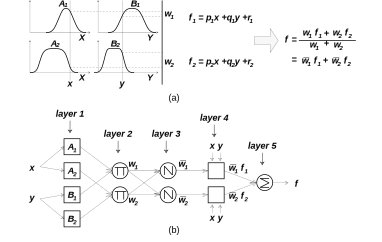
\includegraphics[width=.8\textwidth]{img/anfis}
    \captionsetup{justification=centering}
    \caption{ANFIS mreža koja ostvaruje neizraziti sustav  (slika preuzeta iz \cite{nenr})}
    \label{fig:anfis}
\end{figure}

Prikazana mreža predstavlja sustav koji ima $2$ ulazne varijable $x$ i $y$ te na temelju njih računa rezultat $f$.
Pritom sustav raspolaže sa $2$ pravila, što se na slici vidi kao parovi ($A_1$, $B_1$) i ($A_2$, $B_2$), odnosno $2$ neurona u slojevima $2$, $3$ i $4$.
Kako bi se odredile točne vrijednosti brojeva $A_i$ i $B_i$ definira se funkcija pripadnosti, te je u daljnjem radu korištena sigmoidalna funkcija pripadnosti oblika:
\[
\mu(x) = \frac{1}{1 + e^{b_i(x-a_i)}}.
\]
Korištenjem ove funkcije pripadnosti, svako pravilo ima $2$ parametra za svaku ulaznu varijablu, točnije $a_i$ i $b_i$.
Izgled funkcije u ovisnosti o parametrima prikazana je na slici \ref{fig:sigmoida}.
\begin{figure}[th!]
    \centering
    \begin{subfigure}{.5\textwidth}
        \centering
        \includegraphics[width=.85\linewidth]{img/sigmoida_a}
        \captionsetup{justification=centering}
        \caption{}
        \label{fig:sigmoida_a}
    \end{subfigure}%
    \begin{subfigure}{.5\textwidth}
        \centering
        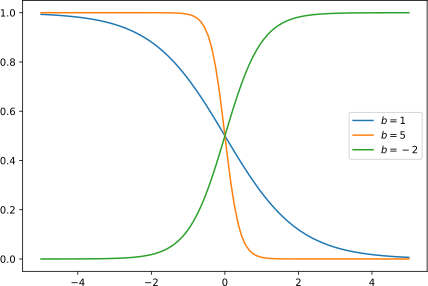
\includegraphics[width=.85\linewidth]{img/sigmoida_b}
        \captionsetup{justification=centering}
        \caption{}
        \label{fig:sigmoida_b}
    \end{subfigure}
    \caption{Graf prijenosne funkcije sa različitim parametrima}
    \label{fig:sigmoida}
\end{figure}
Iz slike \ref{fig:sigmoida_a} može se primjetiti kako parametar $a_i$ zapravo određuje središte sigmoide, odnosno vrijednost $x$ koordinate u kojoj funkcija ima vrijednost $0.5$.
Promjenom ovog parametra, sigmoida se "pomiče" lijevo ili desno.
Na slici \ref{fig:sigmoida_b} prikazano je ponašanje prijenosne funkcije u odnosu na parametar $b_i$ te se može primjetiti kako ovaj parametar određuje strminu funkcije. 
Povećavanjem vrijednosti ovog parametra funkcija postaje strmija, dok se negativnom vrijednosti parametra dobiva zrcalna funkcija.

Vrijednosti neurona u $2.$ računaju se kao $T-$norma, te je za potrebe toga korišten algebarski produkt:
\[
    \mu_{A_i\cap B_i}(x) = \mu_{A_i}(x) \cdot \mu_{B_i}(x).
\]

$3.$ sloj koristi se za normalizaciju vrijednosti prethodnog sloja, te se u njemu računa:
\[
    \bar{w_i} = \frac{w_i}{\sum_{i=1}^{n} w_i}.
\]

U $4.$ sloju računa se vrijednost funkcije uz trenutno pravilo, za dane ulazne vrijednosti.
Korištena je linearna funkcija oblika: 
\[
    f_i = p_i\cdot x + q_i\cdot y + r_i.
\]
Vrijednost funkcije se dodatno množi sa $w_i$ iz prethodnog sloja.
Primjećuje se da su u ovom sloju dodana $3$ nova parametra za svako pravilo, točnije: $p_i$, $q_i$ i $r_i$.

U konačnici se u $5.$ sloju računa konačna vrijednost kao zbroj svih vrijednosti $4.$ sloja.

\section{Izvod algoritma učenja}
Neka je dostupno $N$ primjera za učenje oblika $(\vec{x_i}, y_i)$.
Neka je za neki uzorak $k$ izlaz neuronske mreže označen sa $o_k$, tada se pogreška za taj primjer može definirati kao 
\[
    E_k = \frac{1}{2}(y_k - o_k)^2.
\]

Ako parametre ažuriramo u skladu s algoritmom gradijentnog spusta, za ažuriranje nekog proizvoljnog parametra $\psi$ koristi se izraz:
\[
    \psi(t+1) = \psi(t) - \eta\frac{\partial E_k}{\partial\psi}.
\]

\subsection{Stohastički gradijentni spust}
\subsubsection{Izvod pravila za ažuriranje parametara $p$, $q$ i $r$}
Izlaz sustava definiran je kao težinska suma:
\[
    o_k = \frac{\sum_{i=1}^{m}\alpha_i\cdot z_i}{\sum_{i=1}^{m}\alpha_i},
\]
gdje je $\alpha_i$ jakost paljenja $i-$tog pravila, što je definirano sigmoidalnom funkcijom, odnosno u slučaju ovog konkretnog projekta vrijedi da je:
\[
    \alpha_i = A_i(x_k^{(1)}) \cdot B_i(x_k^{(2)}).
\]
Oznaka $z_i$ jednaka je izračunatoj vrijednosti funkcije za $i-$to pravilo, odnosno:
\[
    z_i = p_i\cdot x_k^{(1)} + q_i\cdot x_k^{(2)} + r_i.
\]
Potrebno je izračunati parcijalnu derivaciju $\frac{\partial E_k}{\partial z_i}$, za što se koristi pravilo ulančavanja:
\[
    \frac{\partial E_k}{\partial z_i} = \frac{\partial E_k}{\partial o_k} \cdot \frac{\partial o_k}{\partial z_i}.
\]
Svaku od dobivenih parcijalnih derivacija moguće je izračunati zasebno:
\begin{equation*}
    \begin{split}
        \frac{\partial E_k}{\partial o_k}
            & = \frac{\partial}{\partial o_k}(
                \frac{1}{2}(y_k - o_k)^2)\\
            & = -(y_k - o_k)
    \end{split}
\end{equation*}

\begin{equation*}
    \begin{split}
        \frac{\partial o_k}{\partial z_i}
            & = \frac{\partial}{\partial o_k}(
                \frac{\sum_{j=1}^{m}\alpha_j\cdot z_j}{\sum_{j=1}^{m}\alpha_j})\\
            & = \frac{\alpha_i}{\sum_{j=1}^{m}\alpha_j}.
    \end{split}
\end{equation*}
Čime se dobije da vrijedi:
\[
    \frac{\partial E_k}{\partial z_i} = -(y_k - o_k)\frac{\alpha_i}{\sum_{j=1}^{m}\alpha_j}.
\]
Kako je već ranije rečeno da vrijedi da je 
\[
    z_i = p_i\cdot x_k^{(1)} + q_i\cdot x_k^{(2)} + r_i,
\]
sad je moguće izračunati parcijalne derivacije po parametrima $p_i$, $q_i$ i $r_i$, čime se dobiju sljedeći izrazi:
\begin{equation*}
    \begin{split}
        \frac{\partial E_k}{\partial p_i}
            & = \frac{\partial E_k}{\partial z_i} \cdot \frac{\partial z_i}{\partial p_i}\\
            & = \frac{\partial E_k}{\partial z_i} \cdot x_k^{(1)}\\
            & = -x_k^{(1)}(y_k - o_k)\frac{\alpha_i}{\sum_{j=1}^{m}\alpha_j},
    \end{split}
\end{equation*}
\begin{equation*}
    \begin{split}
        \frac{\partial E_k}{\partial q_i}
            & = \frac{\partial E_k}{\partial z_i} \cdot \frac{\partial z_i}{\partial q_i}\\
            & = \frac{\partial E_k}{\partial z_i} \cdot x_k^{(2)}\\
            & = -x_k^{(2)}(y_k - o_k)\frac{\alpha_i}{\sum_{j=1}^{m}\alpha_j},
    \end{split}
\end{equation*}
\begin{equation*}
    \begin{split}
        \frac{\partial E_k}{\partial r_i}
            & = \frac{\partial E_k}{\partial z_i} \cdot \frac{\partial z_i}{\partial r_i}\\
            & = -(y_k - o_k)\frac{\alpha_i}{\sum_{j=1}^{m}\alpha_j}.
    \end{split}
\end{equation*}
Iz čega slijede sljedeća pravila za ažuriranje težina:
\begin{equation*}
    \begin{split}
        p_i(t + 1) &= p_i(t) + \eta\cdot x_k^{(1)}(y_k - o_k)\frac{\alpha_i}{\sum_{j=1}^{m}\alpha_j},\\
        q_i(t + 1) &= q_i(t) + \eta\cdot x_k^{(2)}(y_k - o_k)\frac{\alpha_i}{\sum_{j=1}^{m}\alpha_j},\\
        r_i(t + 1) &= r_i(t) + \eta(y_k - o_k)\frac{\alpha_i}{\sum_{j=1}^{m}\alpha_j}.
    \end{split}
\end{equation*}

\subsubsection{Izvod pravila za ažuriranje parametra $a_i$}
Kao i u prethodnom slučaju, potrebno je izračunati parcijalnu derivaciju, što se postiže pravilom ulančavanja:
\[
    \frac{\partial E_k}{\partial a_i} = \frac{\partial E_k}{\partial o_k} 
                                        \frac{\partial o_k}{\partial \alpha_i} 
                                        \frac{\partial \alpha_i}{\partial a_i}.
\]
Komponente su tada redom:
\begin{equation*}
    \begin{split}
        \frac{\partial E_k}{\partial o_k}
            &= -(y_k - o_k),\\
        \frac{\partial o_k}{\partial \alpha_i}
            &= \frac{\partial}{\partial \alpha_i} (\frac{\sum_{j=1}^{m}\alpha_j\cdot z_j}{\sum_{j=1}^{m}\alpha_j})\\
            &= \frac{z_i\sum_{j=1}^{m}\alpha_j - \sum_{j=1}^{m}\alpha_jz_j}{(\sum_{j=1}^{m}\alpha_j)^2}\\
            &= \frac{\sum_{j=1}^{m}\alpha_j(z_i-z_j)}{(\sum_{j=1}^{m}\alpha_j)^2}.
    \end{split}
\end{equation*}
Prije računanja treće parcijalne derivacije uvodi se uznaka $\gamma = -b_i(x-a_i)$, tada vrijedi:
\begin{equation*}
    \begin{split}
        \frac{\partial \alpha_i}{\partial a_i}
            &= \frac{\partial \alpha_i}{\partial \gamma} \cdot \frac{\partial \gamma}{\partial a_i},\\
        \frac{\partial \alpha_i}{\partial \gamma}
            &= \frac{\partial}{\partial \gamma} (\frac {1}{1 + e^{-\gamma}})\\
            &= \frac{\partial}{\partial \gamma} (1 + e^{-\gamma})^{-1}\\
            &= -(1 + e^{-\gamma})^{-2}\cdot (-e^{-\gamma})\\
            &= \frac{e^{-\gamma}}{(1+e^{-\gamma})^2}\\
            &= \frac{1}{1+e^{-\gamma}} \cdot \frac{e^{-\gamma}}{1+e^{-\gamma}}\\
            &= \frac{1}{1+e^{-\gamma}} \cdot (\frac{1+e^{-\gamma}}{1+e^{-\gamma}} - \frac{1}{1+e^{-\gamma}})\\
            &= \frac{1}{1+e^{-\gamma}} (1 - \frac{1}{1+e^{-\gamma}})\\
            &= \alpha_i (1 - \alpha_i),\\
        \frac{\partial \gamma}{\partial a_i}
            &= \frac{\partial}{\partial a_i}(-b_i(x-a_i))\\
            &= \frac{\partial}{\partial a_i}(-b_ix-b_ia_i))\\
            &= b_i,\\
        \frac{\partial \alpha_i}{\partial a_i}
            &= b_i\alpha_i (1 - \alpha_i).
    \end{split}
\end{equation*}

Iz izračunatoga slijedi da se parametar $a_i$ ažurira prema sljedećem pravilu:
\[
    a_i(t+1) = a_i(t) + \eta (y_k - o_k) \frac{\sum_{j=1}^{m}\alpha_j(z_i-z_j)}{(\sum_{j=1}^{m}\alpha_j)^2} b_i\alpha_i (1 - \alpha_i)
\]

\subsubsection{Izvod pravila za ažuriranje parametra $b_i$}
Kod izvođenja pravila za ažuriranje parametra $b_i$ potrebno je odrediti parcijalnu derivaciju:
\[
    \frac{\partial E_k}{\partial a_i} = \frac{\partial E_k}{\partial o_k} 
                                        \frac{\partial o_k}{\partial \alpha_i} 
                                        \frac{\partial \alpha_i}{\partial \gamma}
                                        \frac{\partial \gamma}{\partial b_i}.
\]
Od prije su poznate sve parcijalne derivacije osim $\frac{\partial \gamma}{\partial b_i}$, za koju vrijedi:
\begin{equation*}
    \begin{split}
        \frac{\partial \gamma}{\partial b_i}
            &= \frac{\partial}{\partial b_i}(-b_i(x-a_i))\\
            &= -(x-a_i).
    \end{split}
\end{equation*}
Iz čega slijedi pravilo za ažuriranje parametra $b_i$:
\[
    b_i(t+1) = b_i(t) - \eta (y_k - o_k) \frac{\sum_{j=1}^{m}\alpha_j(z_i-z_j)}{(\sum_{j=1}^{m}\alpha_j)^2} (x - a_i) \alpha_i (1 - \alpha_i)
\]

\subsection{Gradijentni spust}
U postupku gradijentnog spusta potrebno je iyra;unati gradijent za cijeli skup primjera za učenje, zbog čega se greška definira kao:
\[
    E =  \frac{1}{2}\sum_{k=1}^{N}(y_k - o_k)^2,
\]
nakon čega je potrebno sve parcijalne derivacije izračunati u skladu sa ovako definiranom sumom.

\subsubsection{Izvod pravila za ažuriranje parametara}

Potrebno je izračunati parcijalnu derivaciju $\frac{\partial E}{\partial z_i}$, što je jednako:
\begin{equation*}
    \begin{split}
    \frac{\partial E}{\partial z_i} 
        &= \frac{\partial}{\partial z_i} \frac{1}{2}\sum_{k=1}^{N}(y_k - o_k)^2\\
        &= \sum_{k=1}^{N}\frac{\partial}{\partial z_i} \frac{1}{2}(y_k - o_k)^2,
    \end{split}
\end{equation*}
što je zapravo jednako sumi parcijalnih derivacija iz stohastičkog gradijentnog spusta po svim primjerima.
Zbog toga slijedi da je pravilo za ažuriranje parametara:
\begin{equation*}
    \begin{split}
        p_i(t + 1) &= p_i(t) + \eta\sum_{k=1}^{N} x_k^{(1)}(y_k - o_k)\frac{\alpha_i}{\sum_{j=1}^{m}\alpha_j},\\
        q_i(t + 1) &= q_i(t) + \eta\sum_{k=1}^{N} x_k^{(2)}(y_k - o_k)\frac{\alpha_i}{\sum_{j=1}^{m}\alpha_j},\\
        r_i(t + 1) &= r_i(t) + \eta\sum_{k=1}^{N}(y_k - o_k)\frac{\alpha_i}{\sum_{j=1}^{m}\alpha_j}, \\
        a_i(t+1) &= a_i(t) + \eta\sum_{k=1}^{N} (y_k - o_k) \frac{\sum_{j=1}^{m}\alpha_j(z_i-z_j)}{(\sum_{j=1}^{m}\alpha_j)^2} b_i\alpha_i (1 - \alpha_i), \\
        b_i(t+1) &= b_i(t) - \eta\sum_{k=1}^{N} (y_k - o_k) \frac{\sum_{j=1}^{m}\alpha_j(z_i-z_j)}{(\sum_{j=1}^{m}\alpha_j)^2} (x - a_i) \alpha_i (1 - \alpha_i).
    \end{split}
\end{equation*}

\section{Rezultati}
Za potrebe ove vježbe treniran je sustav koji aproksimira funkciju:
\[z = ((x-1)^2 + (y+2)^2 - 5 xy + 3) \cdot \cos(\frac{x}{5})^ 2.\]
\begin{figure}[ht!] 
    \centering
    \includegraphics[width=.65\textwidth]{img/expected}
    \captionsetup{justification=centering}
    \caption{Prikaz grafa funkcije}
    \label{fig:grafFunkcije}
\end{figure}
Na slici \ref{fig:grafFunkcije} prikazan je graf funkcije koju aproksimiramo.
Korištenjem navedene funkcije stvoren je skup podataka za učenje na način da su uzorkovani svi cjelobrojni parovi brojeva iz intervala $[-4, 4]$.
Tako dobiveni brojevi korišteni su za treniranje sustava.
Napravljen je sustav koji koristi $4$ pravila te postiže pogrešku u iznosu $0.14$.
\begin{figure}[ht!] 
    \centering
    \includegraphics[width=.65\textwidth]{img/result}
    \captionsetup{justification=centering}
    \caption{Prikaz grafa funkcije dobivene kao rezultat sustava}
    \label{fig:grafRezultat}
\end{figure}
Slika \ref{fig:grafRezultat} prikazuje graf funkcije koja je dobivena kao rezultat opisanog sustava.

\subsection{Pravilo $1$}
Prvo naučeno pravilo sastoji se od sljedećih težina: 
\[[3.3265, -2.4756, -0.2856, -0.1651, -1.3213, 3.6077, 1.3015].\]
\begin{figure}[th!]
    \centering
    \begin{subfigure}{.5\textwidth}
        \centering
        \includegraphics[width=.9\linewidth]{img/A1}
        \captionsetup{justification=centering}
        \caption{}
        \label{fig:a1}
    \end{subfigure}%
    \begin{subfigure}{.5\textwidth}
        \centering
        \includegraphics[width=.9\linewidth]{img/B1}
        \captionsetup{justification=centering}
        \caption{}
        \label{fig:b1}
    \end{subfigure}
    \caption{Graf funkcija pripadnosti za pravilo 1}
    \label{fig:pripasdnost1}
\end{figure}
Iz slike \ref{fig:pripasdnost1} vidimo grafove funkcije pripadnosti prvog pravila za interval $[-4, 4]$.
Iz slike \ref{fig:a1} vidimo kako je ovo pravilo specijalizirano za velike vrijednosti $x$, odnosno mogli bismo reći "$x$ oko $4$".
Iz slike \ref{fig:b1} vidimo kako je pravilo malo više specijalizirano za veće vrijednosti $y$, no svejedno djeluje i na svim vrijednostima iz intervala.
Konačno područje na kojemu djeluje ovo pravilo prikazano je slikom \ref{fig:podrucje1}.
Funkcija koja je dobivena ovim pravilom prikazana je na slici \ref{fig:rule1}.
\begin{figure}[!ht]
    \centering
    \begin{minipage}{.5\textwidth}
        \centering
        \includegraphics[width=.9\linewidth]{img/ruleArea1}
        \captionsetup{justification=centering}
        \caption{Prikaz područja na kojemu djeluje pravilo 1}
        \label{fig:podrucje1}
    \end{minipage}%
    \begin{minipage}{.5\textwidth}
        \centering
        \includegraphics[width=.9\linewidth]{img/rule1}
        \captionsetup{justification=centering}
        \caption{Prikaz vrijednosti funkcije dobivene pravilom 1}
        \label{fig:rule1}
    \end{minipage}
\end{figure}

\subsection{Pravilo $2$}
Drugo naučeno pravilo sastoji se od sljedećih težina: 
\[[-3.8725, 1.0394, 5.2885, 3.0510, 1.9408, 1.4077, 4.9346].\]
\begin{figure}[th!]
    \centering
    \begin{subfigure}{.5\textwidth}
        \centering
        \includegraphics[width=.9\linewidth]{img/A2}
        \captionsetup{justification=centering}
        \caption{}
        \label{fig:a2}
    \end{subfigure}%
    \begin{subfigure}{.5\textwidth}
        \centering
        \includegraphics[width=.9\linewidth]{img/B2}
        \captionsetup{justification=centering}
        \caption{}
        \label{fig:b2}
    \end{subfigure}
    \caption{Graf funkcija pripadnosti za pravilo 2}
    \label{fig:pripasdnost1}
\end{figure}
Iz slike \ref{fig:pripasdnost1} vidimo grafove funkcije pripadnosti drugog pravila za interval $[-4, 4]$.
Iz slike \ref{fig:a2} vidimo kako je ovo pravilo specijalizirano za manje vrijednosti $x$, odnosno mogli bismo reći "$x$ manje od $-2$".
Iz slike \ref{fig:b2} vidimo kako ovo pravilo podjednako obuhaća sve vrijednosti $y$.
Konačno područje na kojemu djeluje ovo pravilo prikazano je slikom \ref{fig:podrucje2}.
Funkcija koja je dobivena ovim pravilom prikazana je na slici \ref{fig:rule2}.
\begin{figure}[!ht]
    \centering
    \begin{minipage}{.5\textwidth}
        \centering
        \includegraphics[width=.9\linewidth]{img/ruleArea2}
        \captionsetup{justification=centering}
        \caption{Prikaz područja na kojemu djeluje pravilo 2}
        \label{fig:podrucje2}
    \end{minipage}%
    \begin{minipage}{.5\textwidth}
        \centering
        \includegraphics[width=.9\linewidth]{img/rule2}
        \captionsetup{justification=centering}
        \caption{Prikaz vrijednosti funkcije dobivene pravilom 2}
        \label{fig:rule2}
    \end{minipage}
\end{figure}

\subsection{Pravilo $3$}
Treće naučeno pravilo sastoji se od sljedećih težina: 
\[[0.7183, -0.6112, -6.6786, -0.9003, 1.9795, -17.0886, 9.7541].\]
\begin{figure}[th!]
    \centering
    \begin{subfigure}{.5\textwidth}
        \centering
        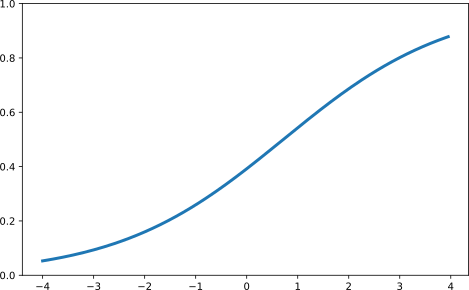
\includegraphics[width=.9\linewidth]{img/A3}
        \captionsetup{justification=centering}
        \caption{}
        \label{fig:a3}
    \end{subfigure}%
    \begin{subfigure}{.5\textwidth}
        \centering
        \includegraphics[width=.9\linewidth]{img/B3}
        \captionsetup{justification=centering}
        \caption{}
        \label{fig:b3}
    \end{subfigure}
    \caption{Graf funkcija pripadnosti za pravilo 3}
    \label{fig:pripasdnost1}
\end{figure}
Iz slike \ref{fig:pripasdnost1} vidimo grafove funkcije pripadnosti trećeg pravila za interval $[-4, 4]$.
Iz slike \ref{fig:a3} vidimo kako je ovo pravilo specijalizirano za veće vrijednosti $x$, odnosno mogli bismo reći "$x$ veće od $0$".
Iz slike \ref{fig:b3} vidimo kako je pravilo jednako specjalizirano za sve vrijednosti $y$.
Konačno područje na kojemu djeluje ovo pravilo prikazano je slikom \ref{fig:podrucje3}.
Funkcija koja je dobivena ovim pravilom prikazana je na slici \ref{fig:rule3}.
\begin{figure}[!ht]
    \centering
    \begin{minipage}{.5\textwidth}
        \centering
        \includegraphics[width=.9\linewidth]{img/ruleArea3}
        \captionsetup{justification=centering}
        \caption{Prikaz područja na kojemu djeluje pravilo 3}
        \label{fig:podrucje3}
    \end{minipage}%
    \begin{minipage}{.5\textwidth}
        \centering
        \includegraphics[width=.9\linewidth]{img/rule3}
        \captionsetup{justification=centering}
        \caption{Prikaz vrijednosti funkcije dobivene pravilom 3}
        \label{fig:rule3}
    \end{minipage}
\end{figure}

\subsection{Pravilo $4$}
Četvrto naučeno pravilo sastoji se od sljedećih težina: 
\[[2.5067, 0.6958, 0.0760, -0.2208, -7.3340, 24.5469, 5.7858].\]
\begin{figure}[th!]
    \centering
    \begin{subfigure}{.5\textwidth}
        \centering
        \includegraphics[width=.9\linewidth]{img/A4}
        \captionsetup{justification=centering}
        \caption{}
        \label{fig:a4}
    \end{subfigure}%
    \begin{subfigure}{.5\textwidth}
        \centering
        \includegraphics[width=.9\linewidth]{img/B4}
        \captionsetup{justification=centering}
        \caption{}
        \label{fig:b4}
    \end{subfigure}
    \caption{Graf funkcija pripadnosti za pravilo 4}
    \label{fig:pripasdnost4}
\end{figure}
Iz slike \ref{fig:pripasdnost4} vidimo grafove funkcije pripadnosti četvrtog pravila za interval $[-4, 4]$.
Iz slike \ref{fig:a4} vidimo kako je ovo pravilo specijalizirano za manje vrijednosti $x$, odnosno mogli bismo reći "$x$ je manje od $2$".
Iz slike \ref{fig:b4} vidimo kako je pravilo malo više specijalizirano za veće vrijednosti $y$, no svejedno djeluje i na svim vrijednostima iz intervala.
Konačno područje na kojemu djeluje ovo pravilo prikazano je slikom \ref{fig:podrucje4}.
Funkcija koja je dobivena ovim pravilom prikazana je na slici \ref{fig:rule4}.
\begin{figure}[!ht]
    \centering
    \begin{minipage}{.5\textwidth}
        \centering
        \includegraphics[width=.9\linewidth]{img/ruleArea4}
        \captionsetup{justification=centering}
        \caption{Prikaz područja na kojemu djeluje pravilo 4}
        \label{fig:podrucje4}
    \end{minipage}%
    \begin{minipage}{.5\textwidth}
        \centering
        \includegraphics[width=.9\linewidth]{img/rule4}
        \captionsetup{justification=centering}
        \caption{Prikaz vrijednosti funkcije dobivene pravilom 4}
        \label{fig:rule4}
    \end{minipage}
\end{figure}

\bibliography{literatura}
\bibliographystyle{plain}
\end{document}